\documentclass{beamer}
\usepackage[T1]{fontenc}
\usepackage{graphicx}
\usepackage{multicol}
\usepackage{listings}
\usepackage{listings,color,xcolor}
%\usepackage{lstlang0}


\usetheme{Berkeley}
\usecolortheme{beetle}

\definecolor{dkgreen}{rgb}{0,0.6,0}

\usepackage{MnSymbol}
\lstset{
	prebreak=\raisebox{0ex}[0ex][0ex]{\ensuremath{\rhookswarrow}},
	postbreak=\raisebox{0ex}[0ex][0ex]{\ensuremath{\rcurvearrowse\space}},
	breaklines=true,
	numbers=left,
	numberstyle=\scriptsize,
	breakatwhitespace=true,
	frame=single,
	frameround=tttt,
	tabsize=4,
	showstringspaces=false,
	aboveskip=1.8em,
	belowskip=0em,
	captionpos=b,
	xleftmargin=0.4em,
	xrightmargin=0em,
	keywordstyle=\bfseries\color{dkgreen},
	commentstyle=\itshape\color{purple},
	identifierstyle=\color{black},
	stringstyle=\color{blue},
	basicstyle=\footnotesize\ttfamily
}

\lstdefinelanguage{Paratype}{
	morekeywords={func,inherits,implements,throws,type,typeclass,contrain,to},
}

\lstdefinelanguage{Go}{
	morekeywords={func, interface, return, int, float, char,
          bool, go, chan, make, new, make, var, true, false},
        morecomment=[l]{//},
        morecomment=[s]{/*}{*/},
        morestring=[b]"
}


\AtBeginSubsection[]
{
  \begin{frame}
    \frametitle{Table of Contents}
    \tableofcontents[currentsection]
  \end{frame}
}

\AtBeginSection[]
{
  \begin{frame}
    \frametitle{Table of Contents}
    \tableofcontents[currentsection]
  \end{frame}
}


\begin{document}

\title[Paratype]{Paratype \\ An Actor Model of Type Evaluation}
\author{Tyler Cecil \\ Christopher Koch \\ Ben Turribiates}
\date{\today}
\institute{New Mexico Tech}

\frame{\titlepage}

\section{The Problem}

\frame {
  \frametitle{What Is Paratype}
}

\frame {
  \frametitle{What is Type Evaluation}
  %Probably need more than one slide here
}


\frame {
  \frametitle{Why do we Need Parallel}
}

\section{Definitions}

%Explain the contexts, trickle up/down, type things, fucking
%everything. Use some of the content from our other slides. DEFINE
%ATLAS AND TYPE MAP, AS WE WILL BE TALKING ABOUT THEM!

\section{Parallelism in GO}

\frame {
  \frametitle{How Does Parallel Work in Golang?}
 
  Paratype was written in \textbf{Google Go}, which gave the program
  interesting and useful properties.

}

\begin{frame}[fragile]
  \frametitle{Go Routines}

  Parallelism in \emph{Go} is based on \emph{Go Routines}. They work
  as lightweight threads. A compiled in scheduler handles the
  concurrency.

  \begin{lstlisting}[language=Go]
func (f *FunctionActor) Run() {
  //Run a function
}
 func Main() {
  f := new(FunctionActor)
  go f.Run()
}
  \end{lstlisting}
\end{frame}

\begin{frame}[fragile]
  \frametitle{Channels}
  
  Communication can occur via \emph{Channels}. Think of them as shared
  memory message queues.

  \begin{lstlisting}[language=Go]
func Sender(ch chan int) {
  msg := 10 
  ch <- msg // send sum to ch
}

func main() {
  ch := make(chan int) // Make a Channel of type 
                       // Int
  go Sender(ch)        // Spawn two go routines
  go Sender(ch)
  x, y := <-ch, <-ch   // Receive from ch
  fmt.Println(x, y, x+y)
}
  \end{lstlisting}
\end{frame}

\begin{frame}[fragile]
  \frametitle{Channels --- Blocking and Non-blocking}

  Channels have a buffer size. Sending a message will only block if
  the buffer is full. Receiving will always block.
  \begin{lstlisting}[language=Go]
// The following are equivalent
ch1 := make(chan int)
ch2 := make(chan int, 0)

// ch3 is a non-blocking channel
ch3 := make(chan int, 128)
  \end{lstlisting}
\end{frame}

\begin{frame}[fragile]
  \frametitle{Messages and Shared Memory}

  Because channels can be freely typed, they can be used to
  communicate shared memory.

  \begin{lstlisting}[language=Go]
// A Channel which sends pointers
ch1 := make(chan *int)

// A Channel which sends other channels
ch2 := make(chan chan int)
  \end{lstlisting}

\vspace{2em}
\emph{Paratype} makes heavy use of this hybrid approach.
\end{frame}


\section{The Parallel of Paratype}

\subsection{Actor Model}

\frame{
  \frametitle{Actor Model}
  \center{\Large So what does it mean that \emph{Paratype}
    
    is an \emph{Actor Model}?}
}

\begin{frame}[fragile]
  \frametitle{Actor Example}

  Consider the following function in the \emph{Paratype} grammar.
  \begin{lstlisting}[language=Paratype]
func f

func q

func g

func h
  \end{lstlisting}
\end{frame}

\begin{frame}[fragile]
  \frametitle{Actor Example}

  \begin{multicols}{2}
    \begin{center}
      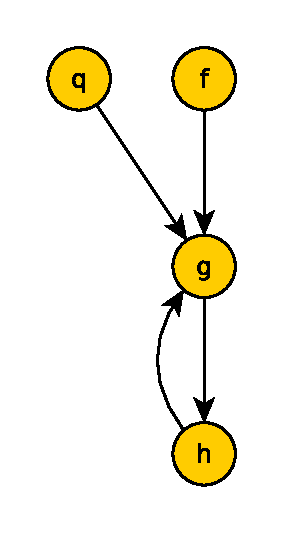
\includegraphics[width=0.7\linewidth]{media/theexamp.eps}
    \end{center}

    \begin{itemize}
      \item This code can be represented by the following \emph{Call
          Graph}.
      \item  When looking at the call graph, we let every node be an 
        \emph{Actor}.
      \item Actors send messages to each other in order to fulfill
        their types. 
    \end{itemize}
  \end{multicols}
\end{frame}

\begin{frame}[fragile]
  \frametitle{Actor Communication --- Hybrid}

  The communication is more complicated than this, however, as data
  needs to be able to \emph{trickle up}.

  \begin{multicols}{2}
    \begin{center}
      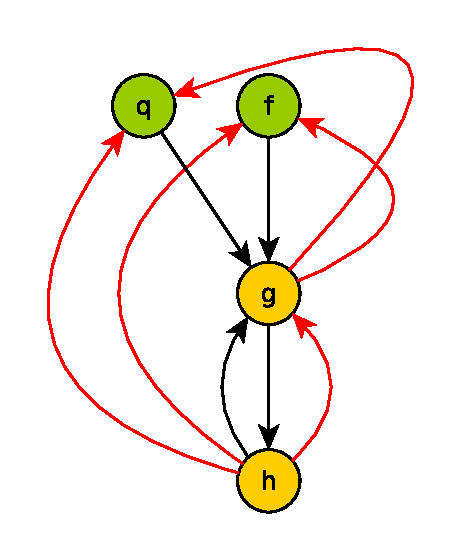
\includegraphics[width=0.7\linewidth]{media/commtypes.eps}
    \end{center}

    \begin{itemize}
      \item {\color{red} Red edges} represent shared memory
        communication.
      \item  Black edges represent sending messages.
      \item {\color{green} Green nodes} represent aristocratic function
      actors.
    \end{itemize}
  \end{multicols}
\end{frame}

\begin{frame}[fragile]
  \frametitle{Actor Routine}
  The Paratype algorithm, at a high level is
  \begin{multicols}{2}
    \begin{enumerate}
      \item Start every function actor.
      \item Function actors build their \emph{context}.
      \item Function actors send their context to their children.
      \item Function actors merge with received contexts.
      \item Function actors send updated messages to their children.
      \item Repeat the last two steps, until a condition is met.
    \end{enumerate}
  \end{multicols}

  Step 4 is a shared memory action, where 3 and 5 are messaging
  actions.
\end{frame}

\subsection{Merging}

%Talk about how merging actually works
%Shared memory, and mutexes!
%For mutexes, mention the Go scheduler.

\subsection{Function Composition}

\begin{frame}
  \frametitle{How Does Function Composition Work}
  
  There is something serious missing in this model: function
  composition is fundamentally different.
\end{frame}

\begin{frame}[fragile]
  \frametitle{Composition Example}

  \begin{multicols}{2}

    We can represent composition with a \emph{Composition Tree}. For
    example:
    

    \begin{lstlisting}[language=Paratype]
q = 
  f(h(g()),h(h(g)),g())
    \end{lstlisting}

    \vspace{2em}
    In this snippet, it is unclear what type variables are being sent
    where.

    \begin{center}
      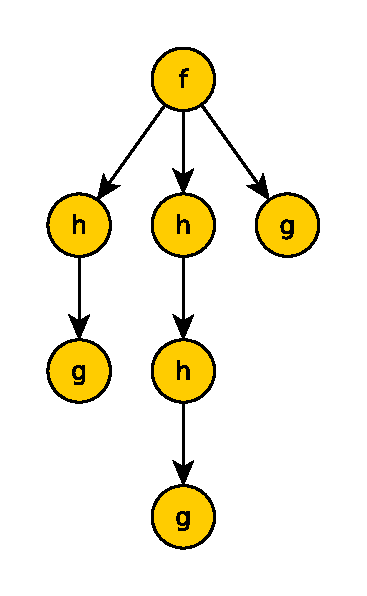
\includegraphics[width=.75\linewidth]{media/composition.eps}    
    \end{center}
  \end{multicols}
\end{frame}

\begin{frame}[fragile]
  \frametitle{In-Out Evaluation}
  \textbf{We must use in-out evaluation!} This is an \emph{inherently
    serial} portion of \emph{Paratype}. The communication requires a
  degree of fines.
\end{frame}

\begin{frame}[fragile]
  \frametitle{Function Composition Procedure}

  If composition is present, the following actions MUST occur:
  \begin{multicols}{2}
    \begin{enumerate}
      \item Send the context to the inner most functions.
      \item Provide a means for those functions to signal when they
        are done.
      \item Repeat with the next layer of functions using more
        up-to-date contexts.
    \end{enumerate}
  \end{multicols}
  We only need to do this once, to gather the relationship between the
  various functions.
\end{frame}

\begin{frame}
  \frametitle{Function Composition Example}
  \centerline{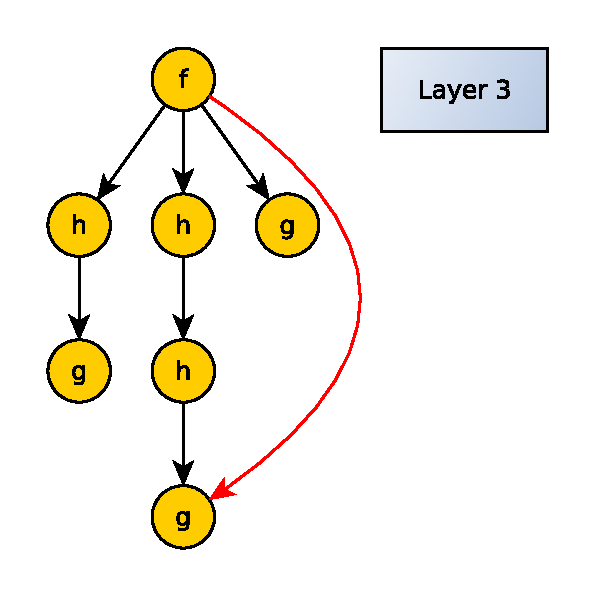
\includegraphics[width=.6\linewidth]{media/inout3.eps}}
\end{frame}

\begin{frame}
  \frametitle{Function Composition Example}
  \centerline{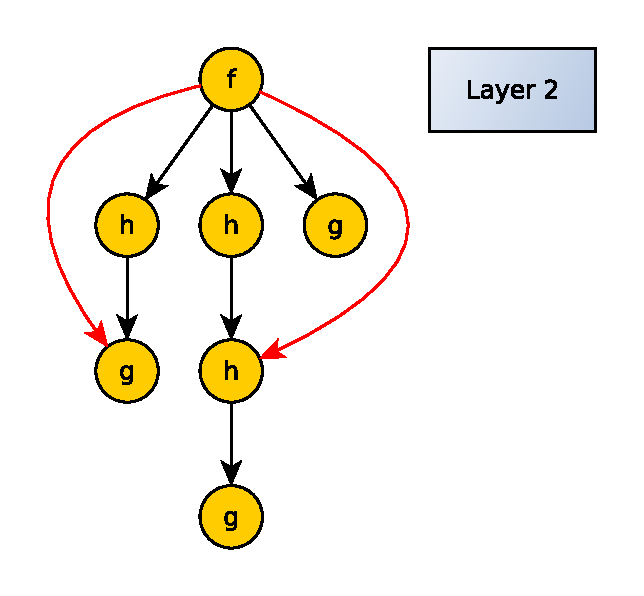
\includegraphics[width=.6\linewidth]{media/inout2.eps}}
\end{frame}

\begin{frame}
  \frametitle{Function Composition Example}
  \centerline{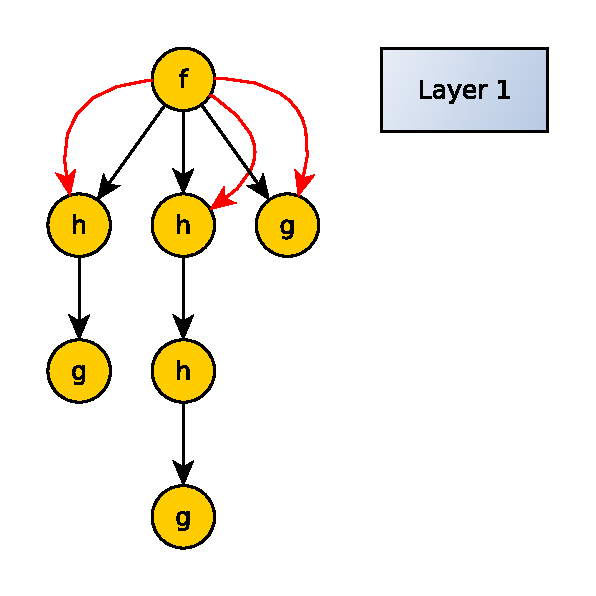
\includegraphics[width=.6\linewidth]{media/inout1.eps}}
\end{frame}

\begin{frame}[fragile]
  \frametitle{WaitGroups}
  
  How does \texttt{f} know when all of a layer has finished? We used a
  Go structure \texttt{sync.WaitGroup} --- similar to a semaphore.

  \begin{lstlisting}[language=Go]
func (wg *WaitGroup) Add(delta int)
func (wg *WaitGroup) Done()
func (wg *WaitGroup) Wait()
  \end{lstlisting}

  \vspace{2em}
  Every child is given a copy of the \texttt{WaitGroup}, and
  decrements it when they are finished. This acts as a barrier for \texttt{f}.
\end{frame}


\subsection{Halting}

%Both normal halting and short circuit halting.

\subsection{Parallel Optimization}

%Lazy Aristocrats
%Catching error types early, by only looking up ONE context treee
%Closing channels as a form of communication

\section{Performance and Analysis}

%Fuck if I know!

\end{document}

%%% local variables: 
%%% mode: latex
%%% tex-master: t
%%% End: e
